\subsection{Discretization of the Controller}\label{ssec:discnController}
The discretization process of a controller consists in using the map from the continuous domain to the discrete domain (z-domain), with respect to the sampling time, \si{T}, of the feedback control system:
%
\begin{flalign} 
  &\si{s = j \omega \to z = e^{s T}}\label{exp:cont2Disc}&
\end{flalign}
%
Since, by definition, the discrete domain cannot represent the complete behavior of a system through time, approximations are used to estimate this behavior. Different methods are briefly described and compared hereafter in this subsection.

The most direct method is the Zero-Order Hold (ZOH) approximation. It mimics a Digital to Analog Converter's output behavior by holding a value of a certain amplitude during a time as long as the defined sampling time. Although, it matches reality correctly as long as the signal does not change too much between each sample, it does not fit as well at high frequencies. Thus, it translates into phase lag in the frequency domain and can cause trouble in closed-loop systems.\\
Another of the most commonly used aproximations is the bilinear transform (or Tustin's method) which is based on the trapezoidal integration principle. A reason to use this method instead of others is that it maps the entire LHP (stable area in the continuous domain) into the unit circle (stable area in the discrete domain)\cite{GFranklin}.\\
The bilinear approximation of \si{z} is defined as:
%
\begin{flalign} 
  &\si{z \approx \frac{1 + s \frac{T}{2}}{1 - s\frac{T}{2}}}\label{exp:bilinearTransform}&
\end{flalign}
%
The inverse transformation of \expr{exp:bilinearTransform} is given by:
%
\begin{flalign} 
  &\si{s \approx \frac{T}{2} \cdot \frac{1 - z^{-1}}{1 + z^{-1}}}\label{exp:inverseBilinearTransform}&
\end{flalign}
%
In general, the \expr{exp:inverseBilinearTransform} is used to replace \si{s} in the continuous-time transfer function of the designed controller. However, due to the non-linear mapping induced by the discretization, a pre-warp of the frequencies can be used before. This avoids effects of phase lag near the cross-over frequency and thus, also avoids unwanted reduction of gain and phase margins, see \cite{GGu,AVOppenheim}. 

Moreover, Matlab has an available function, \lstinline{c2d()}, designed to convert a continuous system's transfer function into the discrete domain by specifying the sampling time (here, \si{T = 0,01s}\fxnote{A justification fo this sampling time should be added at some point.}) and the desired method (\lstinline{'zoh'}, \lstinline{'tustin'} or \lstinline{'prewarp'}). When using the \lstinline{'prewarp'} option, a supplementary argument is needed, corresponding to the critical fequency, see \cite{Matlabc2d}.\\
Here, it is chosen to use \si{33,5\ rad \cdot s^{-1}} as the critical pre-warp frequency, as it corresponds to the point at which the phase lag is at its maximum on the open loop Bode plot of the continuous plant and controller, see \figref{fig:bodeOpenLoopContinuous}.
%
\begin{figure}[H]
  \centering
  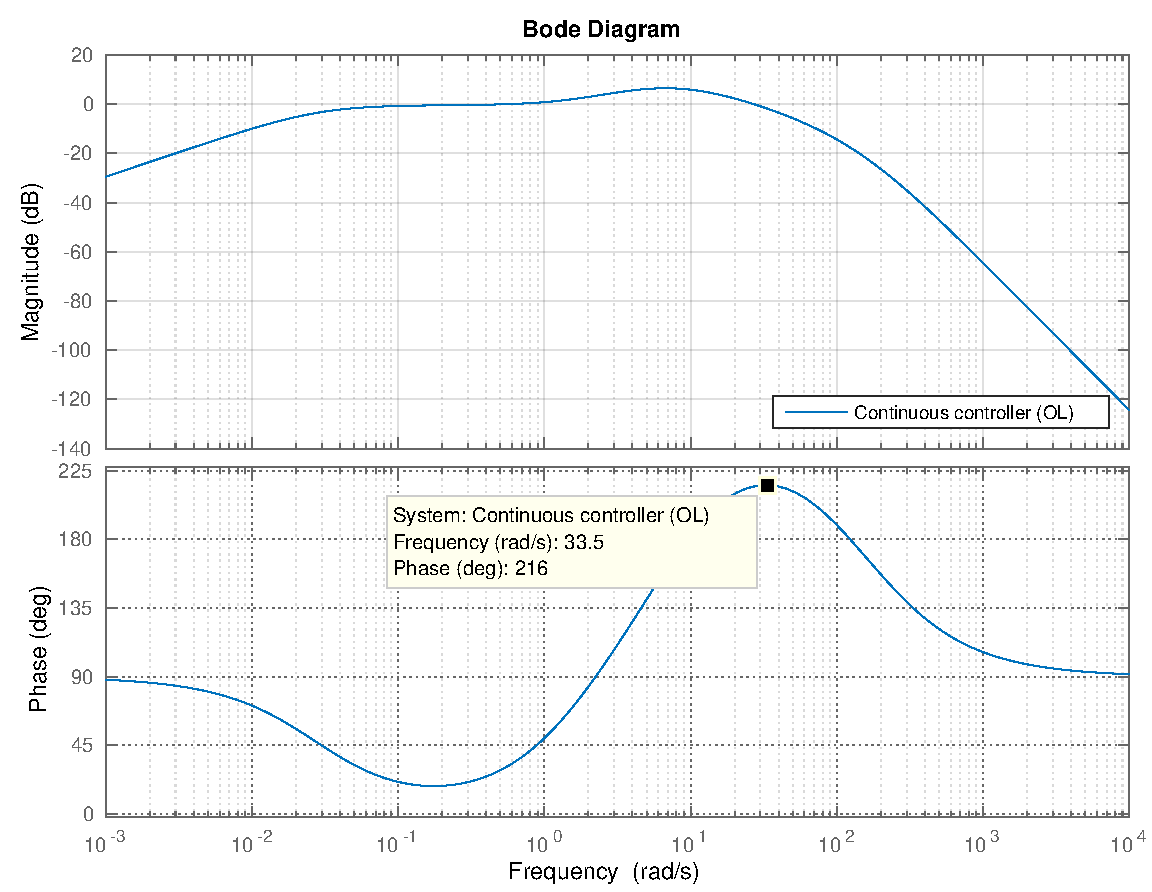
\includegraphics[scale=0.55]{figures/openLoopBadSISOController.pdf}
  \caption{Bode plot of the continuous open loop system}
  \label{fig:bodeOpenLoopContinuous}
\end{figure}
%
\Figref{fig:bodePrewarpVsNoPrewarpVsContinuousOpenLoop} shows Bode plots comparing open loops with the original continuous controller agaisnt the discretized controller's with ZOH, normal Tustin's method and pre-warping, while \figref{fig:bodePrewarpVsNoPrewarpVsContinuousClosedLoop}, shows the system's closed loop responses with these controllers.\\ 
%
\begin{figure}[H]
  \centering
  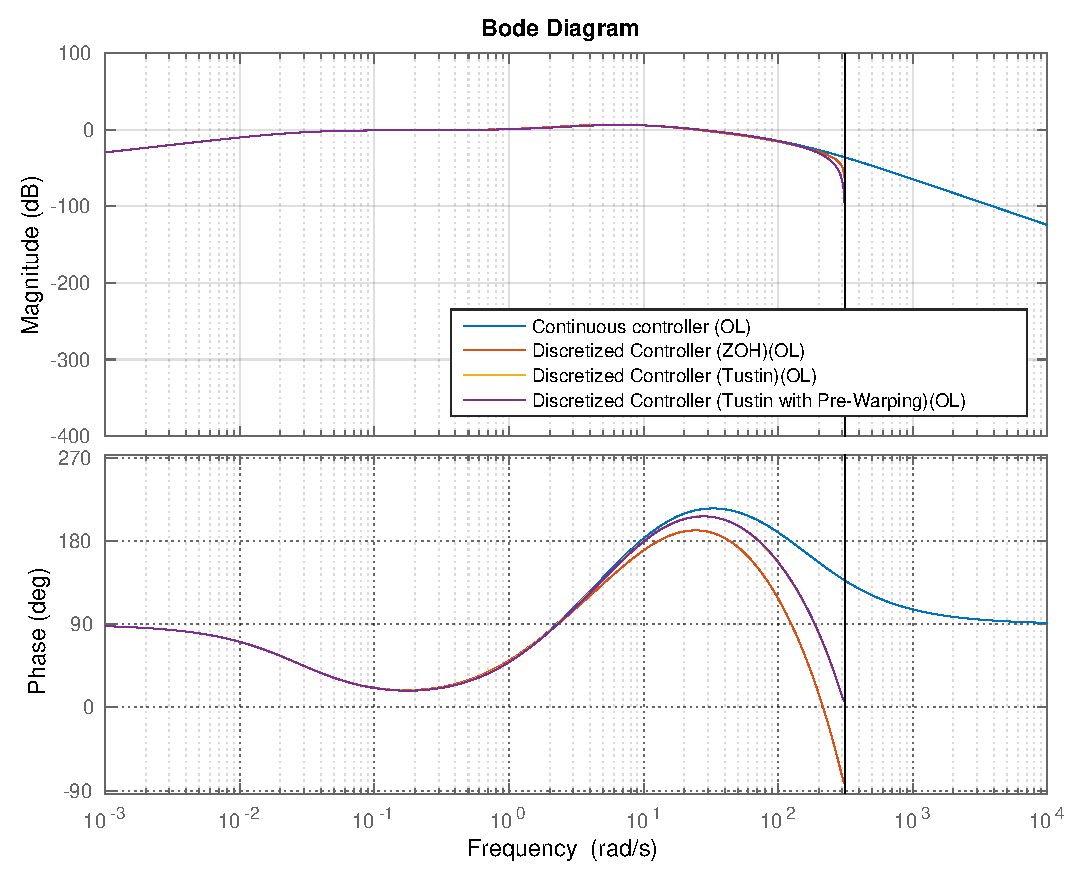
\includegraphics[scale=.6]{figures/zohVsPrewarpVsNoPrewarpVsContinuousBodeOpenLoop.pdf}
  \caption{Bode plot of the open loop system with the continuous controller (in blue), ZOH discretized controller (in red), Tustin discretized controller (in orange) and pre-warped Tustin discretized controller (in purple)}
  \label{fig:bodePrewarpVsNoPrewarpVsContinuousOpenLoop}
\end{figure}
%
From \figref{fig:bodePrewarpVsNoPrewarpVsContinuousOpenLoop}, it is possible to see that the phase of the ZOH discretized controller diverges from the continuous one's, no later than at \si{3\ rad \cdot s^{-1}}. On the other hand, Tustin discretized controllers match closely with the continuous one until approximately \si{10^{1}\ rad \cdot s^{-1}}. \\
The discrete systems here, are only plotted before the vertical line which represents the Nyquist frequency, i.e.~a half of the sampling frequency, chosen earlier in this section\fxnote{If the frequency choic is further explained, the corresponding section should be used as a reference here.}. More importantly, the two discrete versions of the controller, the orange one using a simple Tustin method and the purple one using also pre-warping, seem very similar both in frequency and phase.
%
\begin{figure}[H]
  \centering
  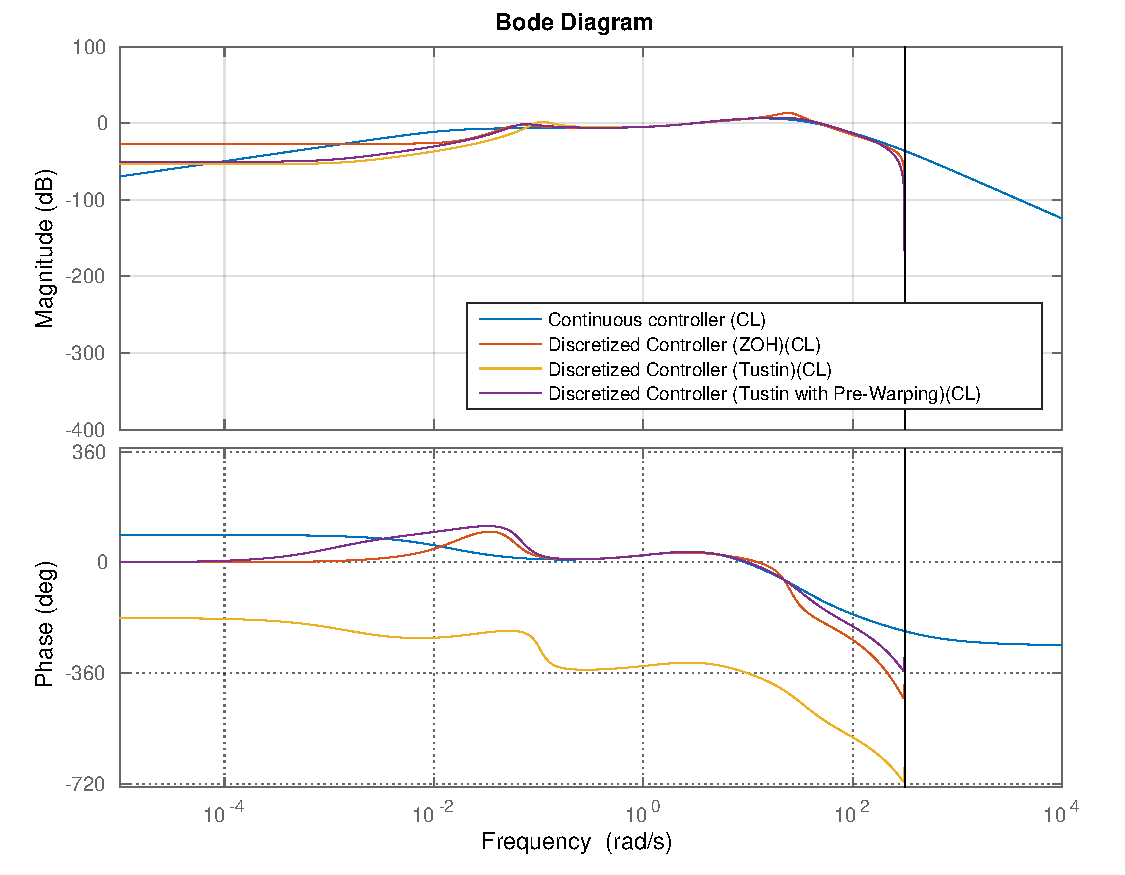
\includegraphics[scale=.6]{figures/zohVsPrewarpVsNoPrewarpVsContinuousBodeClosedLoop.pdf}
  \caption{Bode plot of the closed loop system with the continuous controller (in blue), ZOH discretized controller (in red), Tustin discretized controller (in orange) and pre-warped Tustin discretized controller (in purple)}
  \label{fig:bodePrewarpVsNoPrewarpVsContinuousClosedLoop}
\end{figure}
%
More than with the open loop Bode plot, a difference between controllers is visible by looking at the closed loop Bode plot, on \figref{fig:bodePrewarpVsNoPrewarpVsContinuousClosedLoop}. There, it is apparent that the phase of the pre-warped controller follows more closely the phase of the continuous version than with only Tustin approximation, which is desirable. On the contrary, the non-pre-warped discrete controller has a huge phase lag of at least \si{180^{\circ}} compared to the continuous closed-loop which reveals a substantial delay.\fxnote{Add more to justify pre-warp instead of zoh}

Thus, the pre-warped discretized controller is chosen for the actual implementation on the Cubli, in the code base, see \secref{sec:codeBase}, and its discrete transfer function is:
\begin{flalign}
  \eq{D(z)} {\frac{\tau_{m,w}(z)}{e_{\theta}(z)} = \frac{\num{-8,314} + \num{7,422} \cdot z^{-1} + \num{8,302} \cdot z^{-2} - \num{7,434} \cdot z^{-3}}{1 - \num{1,382} \cdot z^{-1} + \num{0,3415} \cdot z^{-2} + \num{0,001638} \cdot z^{-3}}} &%\unit{N \cdot m} 
  \label{eq:discControllerTf}
\end{flalign}
To implement a discrete controller in a code environment, the preferred form is the difference equation. This is why \eqref{eq:discControllerTf} is transformed into:
\begin{flalign}
  \eqOne{\tau_{m}[n]}{\num{-8,314} \cdot e_{\theta}[n]+ \num{7,422} \cdot e_{\theta}[n-1] + \num{8,3023} \cdot e_{\theta}[n-2] - \num{7,434} \cdot e_{\theta}[n-3] }
  \eqTwo{+ \num{1,382} \cdot \tau_{m}[n-1] - \num{0,3415} \cdot \tau_{m}[n-2] - \num{0,001638} \cdot \tau_{m}[n-3]}\unit{N \cdot m} 
  \label{eq:discControllerDiffEq}
\end{flalign}
%
\hspace{6mm} Where:\\
\begin{tabular}{ p{1cm} l l l}
& \si{\tau_{m}}         & is the wanted motor torque                                      &\unitWh{N \cdot m} \\
& \si{e_{\theta}}         & is the error between wanted and measured frame angle          &\unitWh{rad}\\
& \si{x[n-m]}             & is the m-th previous state of a signal x, m = 0,1,2,3         &\unitWh{\cdot}\\
\end{tabular}

In this subsection, the designed controller has been discretized. The next subsection goes into further analysis of the new feedback control system before the actual implementation on the real system.